 \section{Evaluation}
In this section, we experimentally evaluate our techniques. % demonstrate that context tunneling
% is remarkably effective in practice and our learning algorithm plays a
% key role to achieve the result.
%\myparagraph{Research Questions}
We aim to answer the following research questions:

\begin{itemize}
\item {\bf Effectiveness of context tunneling}: How effective is
  context tunneling in practice? How much does context tunneling
  improve the performance of the state-of-the-art pointer analysis?

\item {\bf Necessity and efficacy of our learning
    approach}:
  Is learning necessary
  to find good context-tunneling heuristics?
  How effectively does the non-greedy algorithm help to find good
  tunneling heuristics?
How sensitive is the
  algorithm to the choice of atomic features?

  % How effectively
  % Does the learning algorithm produce good tunneling heuristics?

% \item {\bf Generality of learned heuristic}: Do the learned heuristics
%   generalize well on unseen programs?%\sehun{other benchmarks}

% \item {\bf Necessity of learning}: Is the learning algorithm necessary
%   to find good heuristics? How does it compare to using simpler approaches?

%   % \item {\bf Compatibility}: Can the idea of context tunneling be
%   %   effectively combined with the existing techniques for achieving
%   %   cost-effective context-sensitivity?

% \item {\bf Impact of using more features}: How sensitive is the learning
%   algorithm to the choice of atomic features? Does using more features
%   help the algorithm to find better heuristics?

%  approach against atomic features with different configurations is?
% \item {\bf Combining with existing approaches}: Can this work be
%   combined with existing approaches for finding good context abstractions
%   such as \cite{JeJeChOh17} or~\cite{TanLX16}?

\item {\bf Learned heuristics}: What insight do the learned
  heuristics provide about context tunneling?

% \item {\bf Adaptability of our learning algorithm}:
%   Performance-oriented context tunneling heuristics or precision-oriented
%   one?
% \item {\bf Simpler tunneling}: How much is $\TunnelingRelation=\langle
%   f_1, f_2 \rangle$ better than more simpler variant
%   $\TunnelingRelation=\langle f_2 \rangle$? For some context sensitivities,
%   a parent method of a method isn't readily available.
%\item \sehun{What else?}
% \item {Other clients or multiple clients}
% \item {Deep context tunneling, i.e.,s2objHT}
% \item {End-to-end comparison with~\cite{TanLX16} and~\cite{JeJeChOh17}}
%\item {Combining with~\cite{JeJeChOh17}}
\end{itemize}



%\subsection{Experimental Setting}

% modified Doop~\cite{TanLX16}
% Java pointer analysis framework. We opt this over the original
% implementation~\cite{Bravenboer2009} because it produces basically same
% analysis results much faster which can accelerate our learning
% process significantly.

\myparagraph{Setting}
We implemented our approach in Doop~\cite{Bravenboer2009},
a widely used framework for pointer analysis for Java~\cite{TanLX16,
  KastrinisS13a, Smaragdakis2011, JeJeChOh17,Tan2017}.
The Doop framework provides four kinds of context-sensitivity:
hybrid context-sensitivity~\cite{KastrinisS13a}, object-sensitivity~\cite{Milanova2002,Milanova2005}, type-sensitivity~\cite{Smaragdakis2011}, and call-site-sensitivity~\cite{Smaragdakis2015}.
Hybrid context-sensitivity is currently considered the state-of-the-art, which
selectively combines object-sensitivity and call-site-sensitivity to
enjoy the benefits of both approaches~\cite{KastrinisS13a}.
Thus, our primary objective is to apply context tunneling to hybrid
context-sensitivity, aiming at advancing the state-of-the-art,
but we also show that context tunneling is useful for
other types of context-sensitivity as well.
% All evaluated analyses used
% 1-context-sensitive heap. For each context-sensitivity flavor, we trained tunneling heuristic
% for depth 1, and compared it with conventional sensitivities of context depth
% 1 and 2.
In short, we consider the
following 12 context-sensitive analyses for Java (all analyses use
1-context-sensitive heap):
\begin{itemize}
	\item Hybrid context-sensitivity\footnote{We write $\onesobjH$ to mean {\it Selective 1-object-sensitive hybrid A} in original paper~\cite{KastrinisS13a}.}:
	\begin{itemize}
		\item \onesobjH,~\twosobjH: 1 and
                  2-hybrid-context-sensitivity with 1
                  context-sensitive heap
		\item \onesobjHT: \onesobjH~with context tunneling
	\end{itemize}
	\item Object-sensitivity:
	\begin{itemize}
		\item \oneobjH,~\twoobjH: 1 and 2-object-sensitivity  with 1
                  context-sensitive heap
		\item \oneobjHT: \oneobjH~with context tunneling
	\end{itemize}
	\item Type-sensitivity:
	\begin{itemize}
		\item \onetypeH,~\twotypeH: 1 and 2-type-sensitivity  with 1
                  context-sensitive heap
		\item \onetypeHT: \onetypeH~with context tunneling
	\end{itemize}
	\item Call-site-sensitivity
	\begin{itemize}
		\item \onecallH,~\twocallH: 1 and
                  2-call-site-sensitivity  with 1
                  context-sensitive heap
		\item \onecallHT: \onecallH~with context tunneling
	\end{itemize}
\end{itemize}

All experiments were done on a machine with Intel i7
CPU and 16 GB RAM running on Ubuntu 14.04 64bit operating system and
JDK 1.6.0\_30.


\myparagraph{Benchmarks}

We used the DaCapo 2006-10-MR2 benchmark suite~\cite{Blackburn2006}, a standard
benchmark for evaluating Java pointer analysis~\cite{
TanLX16,KastrinisS13a, Tan2017,  Smaragdakis2014, JeJeChOh17,  Thiessen2017,   Smaragdakis2011}.
Following~\cite{JeJeChOh17} and~\cite{Smaragdakis2014}, we split ten
programs in DaCapo into 4 small ({\tt luindex}, {\tt
lusearch}, {\tt antlr}, {\tt pmd}) and 6 large ({\tt eclipse}, {\tt
xalan}, {\tt fop}, {\tt chart}, {\tt bloat}, {\tt jython}) programs.
We did not use {\tt hsqldb} because 1-context-sensitive pointer
analysis did not scale (with 5,400s timeout) when a conservative
reflection analysis is used.
On the 4 small programs, we ran our learning algorithm to obtain a
tunneling heuristic for each analysis and then the learned heuristic was
evaluated on the 6 large programs.
For a precision metric, we report the number of type casts proven to be
safe.
% but on average it took 24 hours to learn two Boolean formulas for single
% tunneling heuristic $\TunnelingRelation = \langle f_1, f_2 \rangle$.
%\hakjoo{Report running time in the results}



% \paragraph{\bf Atomic Features}\label{sec:features}

% We used three classes (namely, A, B, and C) of features in Table~\ref{tbl:features}.
% Like other machine-learning approaches, the effectiveness of our
% method depends on the given features. The goal of our learning
% algorithm is to discover a good heuristic by combining atomic
% features rather than to create the heuristic from scratch.
% In this sense, the performance of context tunneling is
% inevitably sensitive to the set of atomic features used. We basically
% use the features in classes A and C, and evaluate the sensitivity to
% features with various combinations of the features.

% Each feature in Table~\ref{tbl:features} describes a syntactic
% property of Java method definitions.  The features are classified into
% three types: signature features (Class A), statement features (Class B), and additional
% features (Class C).  Signature features (A1 -- A10) and statement
% features (B1 -- B15) came from the existing work~\cite{JeJeChOh17} and
% additional features (C1 -- C13) have been newly designed in this work.
% Signature features consist of strings that most frequently appear in
% method signatures from the DaCapo suite. For example, the feature A5
% (``Void'') denotes the set of methods whose signature strings include
% ``Void'' as a substring.  Statement features indicate whether methods
% have a particular type of statement. For example, the feature B10
% denotes the set of methods that contain a conditional statement. These
% (signature and statement) features describe low-level properties of
% methods, which can be easily extracted from programs as already
% available in a Java frontend (e.g. Soot)~\cite{JeJeChOh17}.  On the
% other hand, features A1 -- A13 describe relatively higher-level
% properties, which cannot be expressed by a combination of the previous
% features.  For example, the feature \#11 denotes the set of methods
% that belong to inner classes, i.e., non-static nested classes. Simply
% combining the signature and statement features is not able to describe
% such a property.

% When designing these features, we focused on expressiveness, and
% included a large number of features that can be easily


\subsection{Effectiveness of Context Tunneling}\label{sec:effectiveness-tunneling}

%Let us first demonstrate the effectiveness of context tunneling.
Column \bonesobjHT~of Table~\ref{tbl:sobjobj} presents the highlight
of our results. It shows that context tunneling significantly improves
the precision and scalability of the state-of-the-art hybrid
context-sensitivity.  We generated \onesobjHT~by applying context
tunneling to \onesobjH, where a tunneling heuristic was learned by
running Algorithm~\ref{alg:overall} on the training set of programs
({\tt luindex}, {\tt lusearch}, {\tt antlr}, {\tt pmd}).
Table~\ref{tbl:sobjobj} compares the performance of
\onesobjHT~and~\onesobjH~on both training and test programs.  On the
training set, \onesobjHT~was much more precise and scalable than the
baseline (\onesobjH).  For example, while \onesobjH~analyzes {\tt
  lusearch} in 79s and reports 850 may-fail casts, our analysis with
context tunneling (\onesobjHT) reduces the analysis time and the
number of alarms to 37s and 380, respectively. The improvement
becomes more dramatic in the (larger) test programs. For example,
\onesobjH~reports 2,290 alarms and takes 1,299s in analyzing {\tt
  chart}. Our analysis (\onesobjHT) reduces the number of alarms to
876 while only taking 73s.


Remarkably, \onesobjHT~is even better than
\twosobjH~(2-hybrid-context-sensitivity) in both precision and
scalability on all benchmark programs.  \twosobjH~is currently
considered the state-of-the-art pointer analysis for Java as it
provides most precise results while scaling well to large
programs~\cite{TanLX16,KastrinisS13a,JeJeChOh17}.  Our result
shows that \onesobjHT~can supplant the state-of-the-art. For example, when
analyzing {\tt chart}, \twosobjH~takes 488s and reports 915 may-fail
casts while \onesobjHT~reduces the numbers into 73s and 876,
respectively.  % Indeed, the precision of \onesobjHT~is comparable to
% that of \threesobjH\;(3-hybrid-context-sensitivity with two
% context-sensitive heap), which is generally considered impractical due
% to excessive cost.  \hakjoo{Numbers to justify the previous sentence?}

%In all
%metrics, lower is better. Entries with ``-'' mean that the analysis did not terminate
%within the given time budget (5400 sec.). For precision metrics, we
%count may-fail casts, virtual calls that have multiple targets, and
%reachable methods. For cost metrics, we measure number of
%call-graph edges and analysis time.}

\begin{table}[]
\setlength\extrarowheight{-1pt}
\caption{Effectiveness of context tunneling for hybrid
  context-sensitivity and object-sensitivity.}
\label{tbl:sobjobj}
\centering
\scriptsize
\begin{tabular}{|c| c | l |r| r r  || r | r  r |}
\hline
 &\multicolumn{2}{c|}{\multirow{2}{*}{}} & \multicolumn{3}{c ||}{Hybrid Context
Sensitivity}
  & \multicolumn{3}{c|}{Object Sensitivity}                                                            \\ \cline{4-9}
& \multicolumn{2}{c|}{}                  &\multicolumn{1}{c|}{{\bonesobjHT}}
& \multicolumn{1}{c}{\onesobjH} & \multicolumn{1}{c ||}{\twosobjH} &
\multicolumn{1}{c|}{\oneobjHT} & \multicolumn{1}{c}{\oneobjH} &
\multicolumn{1}{c|}{\twoobjH} \\ \hline


\multirow{16}{*}{\rotatebox[origin=c]{90}{Training programs}}&\multirow{4}{*}{luindex}
                          & \textbf{may-fail casts}& \textbf{371}          & 783        & 415   & 462   & 796 & 496 \\
&                          & \textbf{analysis time(s)} & \textbf{34}           & 66         & 36    & 37    &51 &37  \\
%&                          & poly v-calls     &904                    & 1,117       & 903    & 905 &1,113 & 903      \\
&                          & reachable mthds  & 7,700                 & 7,907       & 7,702  & 7,702 &7,876 & 7,702      \\
&                          & call-graph-edges   & 0.2M                & 0.5M   & 0.9M   &
                          0.3M &0.5M & 1M     \\ \cline{2-9}


&\multirow{4}{*}{lusearch}
                          & \textbf{may-fail casts} &\textbf{380}                & 850        & 420   & 469&812 & 508      \\
&                          & \textbf{analysis time(s)} & \textbf{37}                       & 79        & 63     &41 &56 & 64      \\
%&                          & poly v-calls     &1,077                 & 1,298       & 1,075  &1,078 &1,292 & 1,075      \\
&                          & reachable mthds  & 8,342                & 8,580       & 8,344  &8,344 &8,526 & 8,344      \\
&                          & call-graph-edges  & 0.2M                & 0.5M        & 2M   &0.3M &0.5M & 2.1M      \\ \cline{2-9}


&\multirow{4}{*}{antlr}
                          & \textbf{may-fail casts}  & \textbf{483}                 & 956        & 530   &570 &985 & 611     \\
&                          & \textbf{analysis time(s)} & \textbf{47}                      & 85         & 50   &50 &67 & 45     \\
%&                          & poly v-calls     &1,718                & 1,931       & 1,716  &1,719 &1,927 & 1,716      \\
&                          & reachable mthds  & 8,712            & 8,917      &8 ,714  &8,714 &8,886 & 8,714      \\
&                          & call-graph-edges  & 0.2M            & 0.6M        & 0.9M   &0.3M &0.6M & 1M     \\ \cline{2-9}

&\multirow{4}{*}{pmd}
                          & \textbf{may-fail casts} & \textbf{713}          & 1,217        & 761     &812 &1,210 & 846      \\
&                          & \textbf{analysis time(s)} & \textbf{53}             & 129         & 56     &57 &77 & 57     \\
%&                          & poly v-calls     &946            & 1,185       & 946    &947 &1,171 & 946      \\
&                          & reachable mthds  & 9,086       & 9,322       & 9,090  &9,090 &9,277 & 9,090      \\
&                          & call-graph-edges   & 0.3M       & 0.7M
                                         & 1.3M     &0.3M &0.6M & 1.3M
  \\%\clineB{1-9}{3}
\hline\hline

\multirow{24}{*}{\rotatebox[origin=c]{90}{Testing programs}}&\multirow{5}{*}{eclipse}
                          & \textbf{may-fail casts} & \textbf{586}          &1,061        & 625   &698 &1,092 & 729      \\
&                          & \textbf{analysis time(s)} & \textbf{41}            & 129          & 49    &47 &94 &  51     \\
&                          & poly v-calls     &1,180        & 1,404       & 1,179  & 1,181 & 1,395 &  1,179     \\
&                          & reachable mthds  & 9,195         & 9,461       & 9,188  &9,197 &9,408 & 9,188      \\
&                          & call-graph-edges & 0.3M      & 0.8M      & 1.4M   &0.4M &0.8M & 1.5M      \\ \cline{2-9}

&\multirow{5}{*}{xalan}
                          & \textbf{may-fail casts} & \textbf{572}           & 1,129        & 623  &680 &1,055 & 720     \\
&                          & \textbf{analysis time(s)} & \textbf{64}           & 187         & 465   &400 &179 & 2,047      \\
&                          & \textbf{poly v-calls}     & 1,628        & 1,916       & 1,624  &1,633 &1,861 & 1,628     \\
&                          & reachable mthds  & 10,325       & 10,560      &10,327 &10,336 &10,511 & 10,336    \\
&                          & call-graph-edges & 0.4M         & 1M      & 9M   &1.9M &1M & 35M      \\ \cline{2-9}

&\multirow{5}{*}{fop}
                             & \textbf{may-fail casts} &\textbf{1,080}        & 1,975       & 1,107 & 1,253 & 1,968 & 1,270    \\
&                          & \textbf{analysis time(s)} & \textbf{121}         & 916     & 513    & 176 & 1,797 & 428    \\
&                          & poly v-calls                      & 2,081      & 2,733       & 2,041 & 2,063 &2,650 & 2,047    \\
&                          & reachable mthds               & 14,374     &15,741      & 14,373 & 14,376 & 15,733 & 14,373    \\
&                          & call-graph-edges             & 1M      &3.2M       & 12.1M & 1.6M & 3.9M & 11.4M    \\ \cline{2-9}

&\multirow{5}{*}{chart}
                          & \textbf{may-fail casts} &\textbf{876}        & 2,290        & 915  &1,011 &2,226 & 1,055     \\
&                          & \textbf{analysis time(s)} & \textbf{73}         & 1,299      & 488    &107 &2248 & 316     \\
&                          & poly v-calls     &1,614       & 2,792       & 1,614  &1,616 &2,670 & 1,614     \\
&                          & reachable mthds  &12,503      & 16,037      & 12,510 &12,510 &15,977 & 12,510     \\
&                          & call-graph-edges & 0.5M       & 2.6M       & 11M  & 0.7M & 3.2M & 11.3M     \\ \cline{2-9}

&\multirow{5}{*}{bloat}
                          & \textbf{may-fail casts} & \textbf{1,251}            & 1,931        & 1,326    &1,374 &1,911 & 1,407     \\
&                          & \textbf{analysis time(s)} & \textbf{464}               & 707         & 2,211   &463 &557 & 2,314     \\
&                          & poly v-calls     & 1,668           & 2,075       & 1,650   &1,652 &2,071 & 1,650     \\
&                          & reachable mthds  &9,928      & 10,159     & 9,914  &9,914 &10,116 & 9,914     \\
&                          & call-graph-edges  & 1.4M    & 2.1M      & 35M  &1.4M &1.9M & 35.3M     \\ \cline{2-9}

&\multirow{5}{*}{jython}
                          & \textbf{may-fail casts} & \textbf{837}       & 1,308 &-         &-         &-         &-       \\
&                          & \textbf{analysis time(s)} & \textbf{425}    & 730   &$>$5,400  &$>$5,400  &$>$5,400  &$>$5,400       \\
&                          & poly v-calls           & 1,394          & 1,619     &-         &-         &-         &-       \\
&                          & reachable mthds        & 10,626        & 11,012     &-         &-         &-         &-      \\
&                          & call-graph-edges       & 1.1M            & 2.1M       &-         &-         &-         &-      \\ \cline{1-9}

\end{tabular}
\end{table}

\begin{table}[]
\setlength\extrarowheight{-1pt}
\caption{Effectiveness of context tunneling for type-sensitivity and
	call-site-sensitivity. All
	notations and measures are the same with those in Table~\ref{tbl:sobjobj}.}
\label{tbl:typecs}
\centering
\scriptsize
\begin{tabular}{|c| c | l |r| r r || r | r  r |}
\hline
& \multicolumn{2}{c|}{\multirow{2}{*}{}} & \multicolumn{3}{c ||}{Type
Sensitivity}
  & \multicolumn{3}{c|}{Call-Site Sensitivity}        \\ \cline{4-9}
&\multicolumn{2}{c|}{}                  &
\multicolumn{1}{c|}{\onetypeHT}
& \multicolumn{1}{c}{\onetypeH} & \multicolumn{1}{c ||}{\twotypeH} &
\multicolumn{1}{c|}{\onecallHT} & \multicolumn{1}{c}{\onecallH} &
\multicolumn{1}{c|}{\twocallH} \\ \hline


\multirow{16}{*}{\rotatebox[origin=c]{90}{Training programs}}&\multirow{4}{*}{luindex}
                          & \textbf{may-fail casts} & 575 & 888 & 624 & 784 & 837 & 796\\
&                          & \textbf{analysis time(s)} & 37 & 43 & 34 & 60 & 50 & 348\\
%&                          & poly v-calls     &943 &1,140 & 957&1,052&1,171&1,112     \\
&                          & reachable mthds  & 7,706 & 7,884 & 7,704 & 7,879 & 7,953 & 7,902     \\
&                          & call-graph-edges   & 0.1M & 0.2M & 0.3M & 0.2M & 0.3M & 9.2M   \\ \cline{2-9}


&\multirow{4}{*}{lusearch}
                          & \textbf{may-fail casts} &616 & 926 & 664 & 843 & 938 & 875      \\
&                          & \textbf{analysis time(s)} & 40 & 45 & 36 & 62 & 52 & 364    \\
%&                          & poly v-calls     &1,115 & 1,321 & 1,131 & 1,227 &1,352 &1,293      \\
&                          & reachable mthds  & 8,348 & 8,536 & 8,346 & 8,551 & 8,626 & 8,575    \\
&                          & call-graph-edges  & 0.1M & 0.2M & 0.3M & 0.2M & 0.3M & 9.3M     \\ \cline{2-9}


&\multirow{4}{*}{antlr}
                          & \textbf{may-fail casts}  &707 & 1,061 & 753 & 945 & 1,037&995  \\
&                          & \textbf{analysis time(s)} &59 & 56 & 50 & 98 & 75 & 430    \\
%&                          & poly v-calls     &1,753 & 1,950 & 1,767 &1,862&1,507&1,926      \\
&                          & reachable mthds  &8,718 & 8,894 & 8,716 & 8,885 & 8,961 & 8,910     \\
&                          & call-graph-edges  &0.1M & 0.2M & 0.3M & 0.3M & 0.4M  & 9.5M     \\ \cline{2-9}

&\multirow{4}{*}{pmd}
                          & \textbf{may-fail casts} & 949 & 1,302 & 995 & 1,200 & 1,273 & 1,216      \\
&                          & \textbf{analysis time(s)} & 63 & 65 & 58 & 103 & 78 & 454     \\
%&                          & poly v-calls     &976 & 1,194 & 996 &1,101&1,240&1,180      \\
&                          & reachable mthds  & 9,096 & 9,290 & 9,094 & 9,296 & 9,371 & 9,319      \\
&                          & call-graph-edges   & 0.1M & 0.2M & 0.3M & 0.2M & 0.4M & 9.4M    \\%\clineB{1-9}{4}
\hline\hline
\multirow{24}{*}{\rotatebox[origin=c]{90}{Testing programs}}&\multirow{5}{*}{eclipse}
                          & \textbf{may-fail casts} & 839 & 1,191 & 876 & 1,073 & 1,154 & 1,098     \\
&                          & \textbf{analysis time(s)} &43 & 60 & 45 & 111 & 94 & 574     \\
&                          & poly v-calls     & 1,246 & 1,440 & 1,247 & 1,399 & 1,507 & 1,402     \\
&                          & reachable mthds  & 9,234 & 9,451 & 9,220 & 9,444 & 9,511 & 9,443     \\
&                          & call-graph-edges & 0.2M & 0.3M & 0.4M & 0.3M & 0.4M & 10.5M     \\ \cline{2-9}

&\multirow{5}{*}{xalan}
                          & \textbf{may-fail casts} &907 & 1,229 & 950 & 1,137 & 1,203 & 1,143    \\
&                          & \textbf{analysis time(s)} &75 & 77 & 80 & 142 & 121 & 672     \\
&                          & poly v-calls     & 1,673 & 1,890 & 1,685 & 1,858 & 1,967 & 1,903    \\
&                          & reachable mthds  & 10,383 & 10,560 & 10,375 & 10,539 & 10,613 & 10,560   \\
&                          & call-graph-edges & 0.2M & 0.3M & 0.9M & 0.3M & 0.4M & 9.8M     \\ \cline{2-9}


&\multirow{5}{*}{fop}
                          & \textbf{may-fail casts} & 1,690 & 2,133 & 1,728 & 1,977 & 2,070 & 1,998     \\
&                          & \textbf{analysis time(s)} & 143 & 496 & 212 & 508 & 420 & 3,480   \\
&                          & poly v-calls     & 2,349 & 2,712 & 2,370 & 2,522 & 2,665 & 2,582     \\
&                          & reachable mthds  & 15,386 & 15,794 & 15,363 & 15,108 & 15,217&15,129     \\
&                          & call-graph-edges & 0.6M & 1M & 4M & 0.4M & 0.5M & 10.6M    \\ \cline{2-9}


&\multirow{5}{*}{chart}
                          & \textbf{may-fail casts} &1,451 & 2,449 & 1,502 & 2,376 & 2,485 & 2,410     \\
&                          & \textbf{analysis time(s)} &92 & 422 & 95 & 618 & 400 & 4,339    \\
&                          & poly v-calls     &1,752 & 2,731 & 1,775 & 2,698 & 2,892 & 2,783     \\
&                          & reachable mthds  &13,294 & 16,018 & 13,280 & 16,020 & 16,134 & 16,022     \\
&                          & call-graph-edges &0.2M & 0.6M & 0.8M & 0.4M & 0.6M & 10.7M    \\ \cline{2-9}

&\multirow{5}{*}{bloat}
                          & \textbf{may-fail casts} &1,692 & 2,037  & 1,723 &1,949&2,007&-    \\
&                          & \textbf{analysis time(s)} &71 & 87 & 73 &785&634&$>$5400    \\
&                          & poly v-calls     &1,772 & 2,139 & 1,896 &1,925&2,129&-    \\
&                          & reachable mthds  &9,952 & 10,128 & 9,956 &10,113&10,200&-     \\
&                          & call-graph-edges  &0.3M & 0.3M & 0.8M &0.4M&0.6M&-    \\ \cline{2-9}

&\multirow{5}{*}{jython}
                          & \textbf{may-fail casts} & 1,118 & 1,440 &-  & 1,331 & 1,388 & 1,344      \\
&                          & \textbf{analysis time(s)} & 603 & 431 &$>$5400 & 188 & 163 & 841     \\
&                          & poly v-calls     & 1,459 & 1,665 &- & 1,565 & 1,705 & 1,616       \\
&                          & reachable mthds  & 10,768 & 11,117 &- & 10,987 & 11,066 & 11,006      \\
&                          & call-graph-edges & 0.6M & 0.6M &- & 0.3M & 0.5M & 10M     \\ \cline{1-9}
%\multicolumn{9}{l}{\hakjoo{I deleted this sentence as it reads weird} *We relaxed a cost constraint of the objective function (Section~\ref{sec:opt}) to enable learning.}

\end{tabular}
\end{table}

Note that recent
approaches~\cite{TanLX16,JeJeChOh17} aiming at enhancing \twosobjH~do
so by compromising either precision or scalability.
\cite{TanLX16} presented \Bean, a technique for improving the
precision of object-sensitivity.  \cite{JeJeChOh17} presented a
technique for performing selective context-sensitivity, which applies
context-sensitivity only to a selected set of methods. Both approaches
have been used primarily for improving \twosobjH. However,
\Bean~increases the precision at the expense of scalability~\cite{TanLX16}
and the technique by~\cite{JeJeChOh17} improves the scalability at the
expense of precision. Our analysis, \onesobjHT, increases both the precision and scalability of \onesobjH~at
the same time.



% The results in Table~\ref{tbl:researched} show that our analysis
% (\onesobjHT) establishes a new sweet spot for hybrid
% context-sensitivity. The analysis by~\cite{TanLX16} is more precise
% than $\twosobjH$ at the expense of scalability. The technique
% by~\cite{JeJeChOh17} makes \twosobjH~extremely scalable but it
% sacrifices its precision.
% Our analysis is almost as precise as \cite{TanLX16}
% without compromising scalability too much.




Table~\ref{tbl:sobjobj} and~\ref{tbl:typecs} show that context
tunneling is useful for other types of context-sensitivity as well;
overall, context tunneling enabled 1-object-sensitivity,
1-type-sensitivity, and 1-call-site-sensitivity to perform better than
their counterparts with $k=2$. However, hybrid context-sensitivity
benefitted the most from our technique.
This is because hybrid context-sensitivity provides the best precision
when we use deeper context-sensitivity ($k=2$) in baseline analyses.
Such result implies that we have more chance to find tunneling relations for higher precision than
others.

The results show that context tunneling also improves memory
consumption.
Context tunneling can reduce memory consumption because increased
precision reduces spurious facts (e.g., spurious call-graph
edges). For example, while \oneobjH~generated 0.5 million call-graph edges
for {\tt lusearch}, \onesobjHT~generated 0.2 million edges, confirming
that more than a half of the call-graph edges in the \oneobjH~analysis
are spurious.

% \sehun{The improved precision
% without using deeper contexts resulted more distilled call-graph, too. While conventional \onesobjH~found 0.5 million call-graph edges for {\tt lusearch}, our \onesobjHT~found that more than a half of them are spurious.}
% \sehun{The number of call-graph edges is also consistent with the improvements as ours requires only one-fifth of the conventional analysis's one.}


%; object sensitivity is generally known as better option than call-site one for Java programs and call-site sensitivity covers all method invocations whereas partly due to   All the other
%types of context sensitivity focuses on a single flavor, providing
%less opportunities to benefit from context
%tunneling.
%\minseok{Opportunity: call site = sobj}

 % Note that, in Table~\ref{tbl:sobjobj}, although \onesobjH~and
% \oneobjH~show comparable precision across all benchmarks except for
% {\tt jython}, \onesobjHT~has considerably less alarms than
% \oneobjHT. This is due to the hybrid nature of the baseline context
% sensitivity of~\onesobjH. Unlike \oneobjH~and \onecallH, which only
% consider either of virtual or static method invocations, hybrid
% context sensitivity uses both of them. Our technique is able
% to maximize the potential of \onesobjH by
% generalizing the idea of hybrid context-sensitivity (i.e. which virtual and static methods are ``important'' in
% terms of context generation). \hakjoo{The description here is vague.} \minseok{Tunneling
%   abstration for 1-ctx sensitivity is an approximated tunnel for
%   $k$-ctx sensitivity for $k>1$.}


% Table~\ref{tbl:sobjobj} and~\ref{tbl:typecs} show that our data-driven
% approach can produce context tunneling heuristics that realize
% potential of 1-context-sensitive analyses. Ours consistently preciser
% not only than conventional 1-context-sensitive analyses but also
% comparators with context depth 2. In fact, ours precision figures are
% comparable to ones from 3-context-sensitive analyses, which are
% generally considered as impractical due to their excessive cost. From
% the same tables, we can also conclude that our learning algorithm was
% able to infer general enough heuristics as performance and precision
% figures for testing programs showed similar results with the case of
% training.

% In addition, ours are quicker than conventional analyses with same
% context depth. That means our learning algorithm for tunneling
% heuristic was able to avoid inefficient heuristics due to propagating
% uselessly fine-grained context information throughout the learning
% process.

% Among four context sensitivities, hybrid context sensitivity got the
% most benefit from our approach than the others. In
% Table~\ref{tbl:sobjobj} and~\ref{tbl:typecs}, \onesobjH~and
% \oneobjH~show comparable precision figures across all benchmarks
% except {\tt jython}. However, \onesobjHT~has considerably less alarms
% than \oneobjHT. This result is due to hybrid nature of the base
% context sensitivity~\onesobjH. Unlike \oneobjH~and \onecallH, which
% only consider either of an virtual or static method invocations
% respectively, this hybrid context sensitivity uses both of them. Our
% learning algorithm was able to produce heuristics that maximize
% potential of the \onesobjH by generalizing which virtual and static
% methods were ``important'' in terms of context generation without
% compromise.  \minseok{Tunneling abstration for 1-ctx sensitivity is an
%   approximated tunnel for $k$-ctx sensitivity for $k>1$.}


\subsection{Efficacy of Learning Algorithm}
\label{sec:eval:algorithm}
The key enabler for effective context tunneling is our learning
algorithm.
In this subsection, we discuss our learning
approach from various perspectives. %this perspective.

\myparagraph{Necessity of learning}
One important lesson we learned from this work is that using an automated learning algorithm is essential for
discovering effective tunneling heuristics. Any simple heuristic we
could come up with manually did not achieve good-enough performance.  For
example, we tried all ``single-feature'' heuristics with the
parameters in
$\myset{\langle f_1, f_2 \rangle \mid (f_1 = \false \land f_2 = a)
  \vee (f_1 =a \land f_2 = \false), a \in \afeatures \cup \neg
  \afeatures }$, where $\afeatures$ is the set of atomic features in
Table~\ref{tbl:features}.  Among the 92 ($4 \times |\afeatures|$)
such heuristics, the B1 feature with
$\langle f_1 = \false, f_2 = B1\rangle$ was most effective for the
family of object-based context-sensitivities (i.e. \oneobjH,
\onesobjH, \onetypeH). By using the B1 feature alone, however, we
managed to reduce
the total of 9,694 alarms of \onesobjH~to 7,218 and the analysis time
from 3,968s to 1,367s for the test programs. We failed to
further improve its precision substantially with manual tuning.  On
the other hand, our algorithm effectively refined the feature to the following:
\begin{quotation}
$f_2$: $(\underline{B1} \land B5 \land \neg A6 \land \neg A9 \land \neg B13 \land A1 \land \neg A3) \lor (B9 \land \neg A6 \land A1 \land B5 \land B4 \land \neg B6 \land \neg A9 \land \neg A3 \land \neg A10 \land \neg A4 \land A8 \land \underline{\neg B1}) \lor (B13 \land B5 \land \neg B3 \land \neg A6 \land \neg B9 \land B4 \land \neg A9 \land \neg B10 \land \neg B6 \land \neg A3 \land \neg A5 \land \neg B8 \land A4 \land A8 \land A2 \land B7 \land \underline{\neg B1})$
\end{quotation}
Note that our algorithm not only was able to refine the feature (i.e. the first
conjunct containing $B1$), but also found room for further improvement
with $\neg B1$ (i.e. the second and third conjuncts). With this
refinement, the precision of the heuristic improved significantly,
reducing the number of alarms from 7,218 to 5,202, finally
outperforming $\twosobjH$.  Discovering such a
complex heuristic manually is totally nontrivial for real-world
programs.

\myparagraph{Impact of non-greedy strategy}

% A key enabler for effective heuristics was the ability of
% the algorithm to explore the search space in a non-greedy manner.
Our algorithm is able to find a good heuristic because it explores the
search space in a non-greedy manner.
That is, it seeks to maximize
the final performance of heuristics rather than blindly pursuing the immediate improvement.
To see the impact of this strategy, we compared our algorithm against
a greedy algorithm that maximizes the immediate benefit.
We made this greedy version of our algorithm by modifying the
$\ChooseSeed$ and $\HasSeed$ functions, so that they measure
the potential of a heuristic based on the total number of proved
queries, not on the number of
{\em exclusively} proved queries. Precisely, the $\ChooseSeed$ is redefined as in Eq.~\ref{eq:greedy-choose-seed} and the $\HasSeed$ is changed to return $\true$ always.
With this strategy, the learning algorithm becomes to always favor
a parameter that maximally improves the current heuristic; it never
explores parameters that are worse than the current one.

Figure~\ref{fig:greedy} shows that our non-greedy strategy has
significant impact on the final quality of learned heuristics.
It depicts how the precision of the current
heuristic changes over time during the learning
algorithm.  The x-axis reports progress of the learning procedure\footnote{We collected refinements that passed the condition at line 10 in Algorithm~\ref{alg:learning} for better understanding.} and
the y-axis reports the precision in terms of the number of unproven 
queries on the training set of programs (lower is better). Note that
our algorithm (black solid line) repeatedly explores parameters that
are much worse than the current one but doing so enables to find a good
parameter in the end. With the greedy strategy (red dotted line), the
algorithm converges to suboptimal outcomes. Crucially, the heuristics
learned by this greedy algorithm could not beat the conventional
2-context-sensitive approaches on test programs. 

\begin{figure}[t]
  \centering
  \begin{subfigure}[b]{.48\textwidth}
  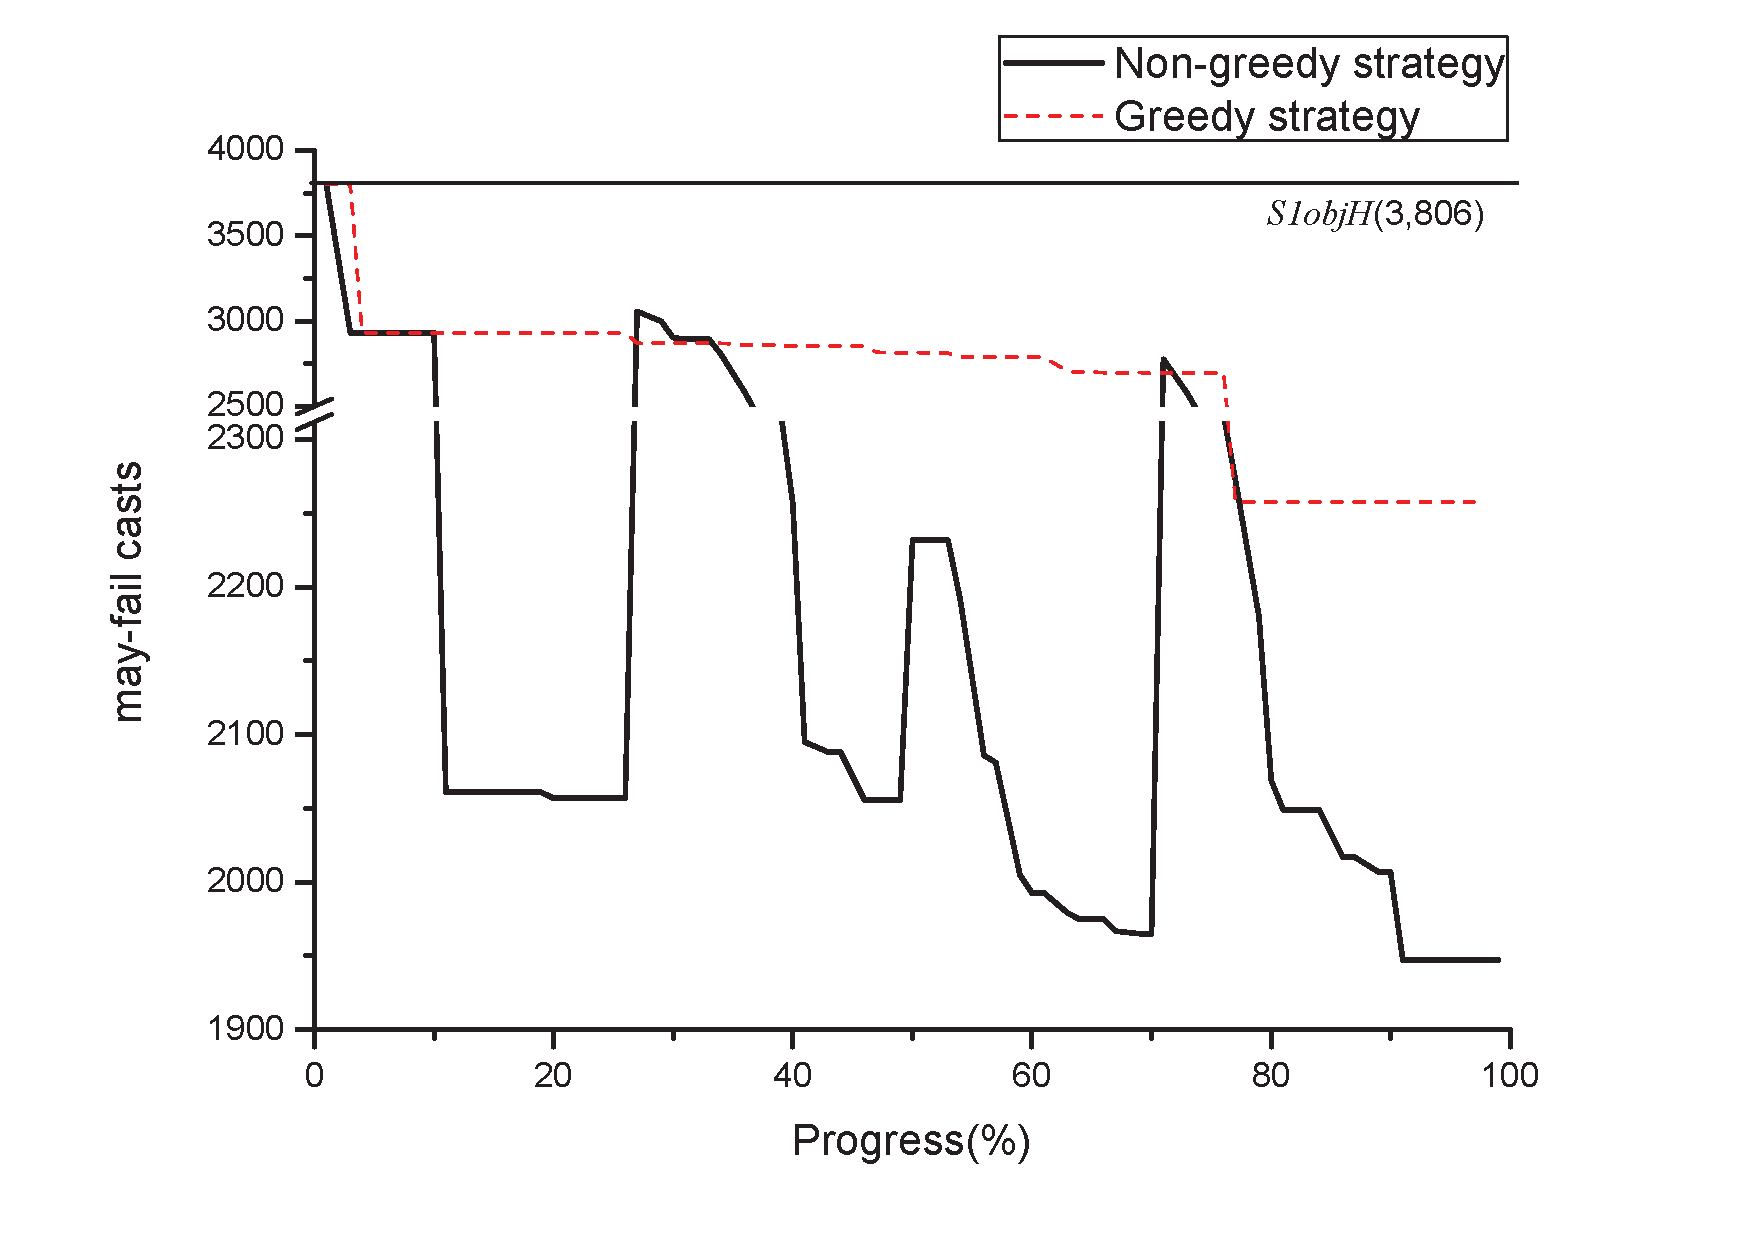
\includegraphics[width=\textwidth]{ContextTunneling/figures/sobj_ours_greedy.pdf}
  \caption{Hybrid context-sensitivity}
  \label{fig:greedy_sobj}
  \end{subfigure}
  ~
  \begin{subfigure}[b]{.48\textwidth}
  \includegraphics[width=\textwidth]{ContextTunneling/figures/type_ours_greedy.pdf}
  \caption{Type-sensitivity}
  \label{fig:greedy_type}
  \end{subfigure}
  \caption{Impact of our non-greedy learning strategy.
% Changes of parameter's precision over time. We have two cases; hybrid context sensitivity and type sensitivity. X-axis is learning progress and Y-axis is a number of casting failure alarms (lower is better). The plots have additional horizontal lines that denote the precisions of conventional analyses, $\onesobjH$ and $\onetypeH$ respectively, to provide readers comprehensive view. Solid black lines are for our learning algorithm and red dotted lines are for ours without considering exploration.
}
  \label{fig:greedy}
\end{figure}


\myparagraph{Generality of learned heuristics}
The algorithm is able to learn
heuristics that do not overfit to training data and generalize well to
unseen programs.
Tables~\ref{tbl:sobjobj} and~\ref{tbl:typecs} show that
the context-tunneling heuristics learned with the small programs ({\tt
  luindex}, {\tt lusearch}, {\tt antlr}, {\tt pmd}) in the DaCapo
suite perform well on the large programs ({\tt eclipse}, {\tt xalan},
{\tt fop}, {\tt chart}, {\tt bloat}, {\tt jython}). We also checked
the generality of the heuristics beyond the DaCapo benchmarks.
We evaluated the learned heuristic for \onesobjHT~on two large applications,
{\tt JPC}\footnote{\url{http://jpc.sourceforge.net/home_home.html}} and {\tt checkstyle}\footnote{\url{http://checkstyle.sourceforge.net}}. Table~\ref{tbl:other-benchmarks} shows
that our heuristic substantially outperforms both \onesobjH~and
\twosobjH~for these programs.


\begin{table}[t]
\small
\centering
\caption{Generalization to other benchmarks}
\label{tbl:other-benchmarks}
\begin{tabular}{lrrrrrr}
  \toprule
  \multirow{2}{*}{Benchmarks} & \multicolumn{2}{c}{\onesobjHT} &
                                                                \multicolumn{2}{c}{\onesobjH} &\multicolumn{2}{c}{\twosobjH} \\
  \cmidrule(lr){2-3} \cmidrule(lr){4-5} \cmidrule(lr){6-7}
  & may-fail casts & time(s) & may-fail casts & time(s) & may-fail casts & time(s)\\
  \midrule
  JPC &1,593 &230 & 2,595 &2,578 &1,627 &1,597\\
%  fop & 1,975 & 1,119 & 1,095 & 181 & &\\
  checkstyle &474 &80 &902 &111 &508 &158\\
  \bottomrule
\end{tabular}
\end{table}
%\hakjoo{Include S2objH results in the table above}



%\hakjoo{Describe benchmarks and results}



% \begin{tabular}{|c|c|c|c|c|}
% \hline
% \multirow{2}{*}{s1objT} & \multicolumn{2}{c|}{non-greedy}                       & \multicolumn{2}{c|}{greedy}                           \\ \cline{2-5}
%                   & alarm                      & cost                     & alarm                      & cost                     \\ \hline
% bloat             & \multicolumn{1}{r|}{1,251} & \multicolumn{1}{r|}{456} & \multicolumn{1}{r|}{1,302} & \multicolumn{1}{r|}{428} \\ \hline
% \end{tabular}

% We made two changes in order to make the comparator. First, we modified $\ChooseSeed$ function, which returns an atomic feature to refine, to consider overall provable queries per se, not the potential. More precisely, we redefined the function as follows:
% \[
% \ChooseSeed(i,\params, F, \vec{P}, W)=\argmax_{a\in W}{\sum\limits_{P\in \vec{P}}{\lvert \precision(F_P(\heuristic_{\params{[f_i \mapsto \myset{\myset{a}}]}}(P)))}\rvert}
% \]
% Next, the comparator also focuses on overall precision gains only when evaluate each refinement step. Specifically, we replaced Algorithm~\ref{alg:learning-inner}'s conditional statement for the evaluation (line 15 -- 21) with following lines:
% \begin{center}
% \small
% 	\begin{algorithmic}[1]
%     \setcounterref{ALG@line}{alg:if}
%   	        \If {$(\PrecP(\params', \params'', \vec{P}) \lor \PrecE(\params', \params'', \vec{P})) \land \CostM(\params', \params'', \vec{P})$} \Comment{no longer consider \HasSeed}
%   	          \State $c \gets c'$
%             \Else
%               \State $\Failed \gets \Failed \cup a$ \Comment{record the failed attempt}
%   	        \EndIf
% 	\end{algorithmic}
% \end{center}
% All in all, the comparator always chooses the most promising atomic features with regard to overall precision gains and accepts any refinements if they made analysis more precise than before. In other words, the comparator makes decisions without knowing where the precision gains come from. Therefore, it misses opportunities for chasing queries that conventional analysis can't and results suboptimal context tunneling heuristics.


% We illustrate the impact of exploration in Figure~\ref{fig:greedy} using $\onesobjHT$ and $\onetypeHT$. In both cases, ours (black solid lines) finds desirable solutions by going back and forth repeatedly while the comparator (red dotted lines) reaches suboptimal solutions with more consistent manner.

% \begin{figure}[t]
% \begin{center}
%   \includegraphics[scale=0.35]{figures/type_ours_greedy.pdf}
% \end{center}
% \caption{Impact of our non-greedy learning strategy. }
% \label{fig:greedy}
% \end{figure}





%\subsection{Sensitivity to Atomic Features}\label{sec:eval-features}
\myparagraph{Impact of using more features}

%We used three classes (namely, A, B, and C)  of features in
% Like other machine-learning approaches, the effectiveness of our
% learning algorithm depends on the given features. The goal of our learning
% algorithm is to discover a good heuristic by combining atomic
% features rather than to create the heuristic from scratch.
% In this sense, the performance of context tunneling is
% inevitably sensitive to the set of atomic features used. We basically
% use the features in classes A and C, and evaluate the sensitivity to
% features with various combinations of the features.

Our algorithm is likely to produce a better heuristic as more diverse
features are used. %  Like other machine-learning approaches, the
% effectiveness of our learning algorithm depends on the given
% features.
We evaluated our algorithm with 1) the A features only, 2) the B
features only, and 3) the A and B features.  We learned a heuristic for
each set of features from the training programs, and then evaluated
its performance on the test programs.  Table~\ref{tbl:sens_afest}
presents the results.  Overall, using all of the A and B features was
most effective.  The high-level features (B) primarily helped to
increase the precision of the learned heuristic. However, using the B
features alone was unable to find scalable heuristics.  Additionally using the
low-level features (A) enabled the algorithm to refine the B features
delicately, generating a heuristic outstanding in both precision and scalability.
% scalable heuristics.
% Even with the A features only, the algorithm found a heuristic more precise than the conventional analysis
% (i.e. $\onesobjH$).
% Additionally using the B features helped to reduce the analysis time.
% Inclusion of the C features enabled the algorithm to find a more
% precise heuristic.
% \hakjoo{Revise this paragraph }

% but using a
% combination of signature features (class A) and additional features
% (class C) resulted the best heuristic of all. Replacing the additional
% features with statement features (class B) resulted a slightly faster
% but substantially less precise heuristic. The precision and cost
% worsen even further when we excluded the statement features and used
% signature features only. The results show that inclusion of the
% additional features...

\begin{table}[]
\small
\centering
	\caption{Impact of using more features}
	\label{tbl:sens_afest}
	\centering
	\begin{tabular}{l r r r r r r r r}
		\toprule
		\multirow{2}{*}{Benchmarks} &
        \multicolumn{2}{c}{Baseline(\onesobjH)} &
                                                    \multicolumn{2}{c}{With
                                                  A only}
          & \multicolumn{2}{c}{With B only} &
                                                      \multicolumn{2}{c}{With
                                                      A and B } \\%With the single feature C1}\\
		\cmidrule(lr){2-3} \cmidrule(lr){4-5}   \cmidrule(lr){6-7} \cmidrule(lr){8-9}
		& alarms                          & time(s) & alarms                  & time(s) & alarms & time(s) & alarms & time(s) \\
		\midrule
		eclipse   & 1,061     & 129   & 807   & 69    & 583    & 47    & 586   & 41  \\%& 814     & 48 \\
		xalan     & 1,129     & 187   & 866   & 179   & 585    & 137   & 572   & 64  \\%& 896     & 90\\
		fop       & 1,975     & 916   & 1,250 & 179   & 1,102  & 163   & 1,080 & 121  \\%& 1,306   & 115\\
		chart     & 2,290     & 1,299 & 1,200 & 120   & 887    & 98    & 876   & 73  \\%& 1,306   & 115\\
		bloat     & 1,931     & 707   & 1,634 & 1,156 & 1,250  & 548   & 1,251 & 464 \\%& 1,595   & 534\\
		jython    & 1,308     & 730   & 1,039 & 379   & 844    & 3,747 & 837   & 425 \\%& 1,068   & 412\\
		% \midrule
		% luindex     &783 &66 & 371   &30  & 537     & 66 &379 &40\\%& 1,306   & 115\\
		% lusearch     &850  &79  & 380 & 35 & 572 & 66 &389 &44\\%& 1,306   & 115\\
		% antlr     &956 &85 & 438 & 49 & 683  & 80 &490 &51\\%& 1,595   & 534\\
		% pmd    &1,217  &129 & 713 & 52 &921 &86 &720 &60\\%& 1,068   & 412\\
\hline
		\textsc{Total} & 9,694 & 3,968 & 6,796  & 2,082 &5,251 & 4,740 & 5,202  & 1,188\\
		\bottomrule
	\end{tabular}
\end{table}


\myparagraph{Learning cost}


Our learning algorithm took 53 -- 137 hours to generate the heuristics
used in Table~\ref{tbl:sobjobj} and~\ref{tbl:typecs}. For hybrid
context-sensitivity, it took 57 hours in total (21 hours for
generating the parameter $f_1$ and 36 hours for $f_2$).  For
object-sensitivity, the algorithm required 26 hours for $f_1$ and 28
hours for $f_2$. For type-sensitivity, it took 76 hours for $f_1$ and
61 hours for $f_2$.  For call-site-sensitivity, the algorithm took 53 hours in total (24 hours for $f_1$ and 29 hours for $f_2$). Our algorithm was most
expensive for type-sensitivity because it found relatively a large set
of seed
features and required more iterations to refine all of them (see
Figure~\ref{fig:greedy_type}). % shows that our algorithm
% refined those identified seed features to find complex but more
% optimal solution as in Appendix~\ref{app:formulas:type} than the
% baseline.

Our algorithm is expensive, but it is useful because learning occurs
off-line and only consumes machine-time. In particular, generating
such a heuristic manually would require much more expensive human
costs. Nonetheless, we could reduce the learning cost by
approximation.
One possible way is to only learn the formula $f_2$ and then merely
set $f_1$ to $\false$. The resulting parameter $\langle \false, f_2
\rangle$ makes the heuristic less discerning, giving sub-optimal
results, but the learning cost can be halved.
Table~\ref{tbl:f2} shows this trade-off between learning cost and
optimality.
Overall, \onesobjHT~learned with the approximate learning is less precise and
slightly faster than the analysis with full learning.



\begin{table}[]
\small
\centering
	\caption{Tradeoff between learning cost and performance. % \sehun{Gap between two configurations looks less significant (159 alarms in total). Instead of reporting full figures, just mentioning the most significant case (i.e., bloat) seems good for us.}
        }
	\label{tbl:f2}
	\centering
	\begin{tabular}{c c r r r r r r r}
		\toprule
		  &Learning Cost &                          & eclipse & xalan & fop  & chart & bloat & jython \\ \midrule

		 Full learning   & \multirow{2}{*}{54 hours} & alarms & 586     & 572   & 1,080 & 876   & 1,251  & 837    \\
		($\langle f_1,f_2\rangle$)& &time(s)   & 41      & 64    & 121  & 73    & 464   & 425    \\ \midrule
		Approximate  & \multirow{2}{*}{29 hours} &alarms & 605     & 588   & 1,099 & 897   & 1,317  & 855    \\
		($\langle \false,f_2\rangle$)&& time(s)   & 33      & 54    & 90   & 57    & 335   & 367    \\ \bottomrule
	\end{tabular}
\end{table}



\subsection{Learned Heuristics}\label{sec:tunneling:learnedHeuristics}
The learned heuristics hint at when
and where context tunneling is useful in practice.
For example, our learning algorithm automatically discovered the
characteristics of methods
that benefit from deeper ($k \ge 2$) object-sensitivity, which was
originally conjectured by \cite{Milanova2005}.
\cite{Milanova2005} stated that deeper object-sensitivity may be
useful for methods that belong to sub-objects.
Consider the code snippet % we arranged from the original paper's description
that defines a composite class using a sub-object:
\lstset{
 language=Java,
 aboveskip=3mm,
 belowskip=3mm,
 showstringspaces=false,
 columns=flexible,
 basicstyle={\small\ttfamily},
 numbers=left,
 numbersep=5pt,
 numberstyle=\small\color{gray},
 keywordstyle=\color{blue},
 commentstyle=\color{dkgreen},
 stringstyle=\color{mauve},
 breaklines=true,
 breakatwhitespace=true,
 tabsize=3,
 xleftmargin=5.0ex
}
\begin{lstlisting}
class A {} class B {}
class SubObject {
 Object id(Object v) { return v; }
}
class CompositeClass {
 public SubObject att;
 public CompositeClass(){
   att = new SubObject();//SO
 }
}
class Main{
 public static void main(String[] args){
   CompositeClass cc1 = new CompositeClass();//CC1
   CompositeClass cc2 = new CompositeClass();//CC2
   A a = (A)cc1.att.id(new A());//Query 1
   B b = (B)cc2.att.id(new B());//Query 2
 }
}
\end{lstlisting}
To prove the safety of two down-casting queries at lines 15 and 16,
two method calls to {\tt id} should be analyzed separately.
However, object-sensitivity with $k=1$ fails to prove the queries
because the analysis merges the two contexts into the same context $[\texttt{SO}]$. On the other hand, deeper object-sensitivity (e.g., $k = 2$) can accommodate
the composite class's allocation sites along with the one of
sub-objects ($[\texttt{CC1}, \texttt{SO}]$ and $[\texttt{CC2},
\texttt{SO}]$), concluding that each invocation of \texttt{id} returns one of \texttt{A} or \texttt{B}, not both. Here, we can apply context tunneling instead of using deeper context; the
sub-objects' method should inherit the context from the parent method, i.e.,
the constructor of \texttt{CompositeClass}, instead of updating the
context. In other words, contexts of the constructor \texttt{CompositeClass} are {important} and they should be propagated without modification.
By doing so, object-sensitivity with $k=1$ and context tunneling can prove the queries.
Our learning algorithm captured this situation automatically.
It produced the $f_1$ formula for object-sensitivity
with the following conjunction:
\begin{quotation}
 $\cdots \lor (A8 \land B5 \land \neg B3 \land A1 \land \neg A6 \land \neg A3 \land \neg B9 \land B4 \land \neg A9 \land \neg B11 \land \neg A2 \land \neg B7 \land \neg B1 \land \neg B8 \land \underline{B12} \land \underline{B10} \land \neg B13 \land \underline{B6} \land A5 \land \underline{A10} \land A7 \land \neg A4)$
\end{quotation}
Note the four underlined atomic features: $A10$ for constructor
methods, $B12$ and $B10$ for methods with heap allocations, and $B6$
for methods containing field store. Combining these features denotes a
set of constructor methods that allocate heaps inside and store
something into their member attributes, which describes methods such
as one given above.  



%%% Local Variables:
%%% mode: latex
%%% TeX-master: "paper"
%%% End:
